\documentclass{article}
\usepackage[utf8]{inputenc}
\usepackage{amsmath}
\usepackage{pgfplots}
\pgfplotsset{compat=1.9}
\usepackage{amssymb}
\usepackage{xcolor}
\usepackage{tikz}
\usetikzlibrary{decorations.markings,arrows,calc,intersections}
\usepackage[T1]{fontenc}

\begin{document}

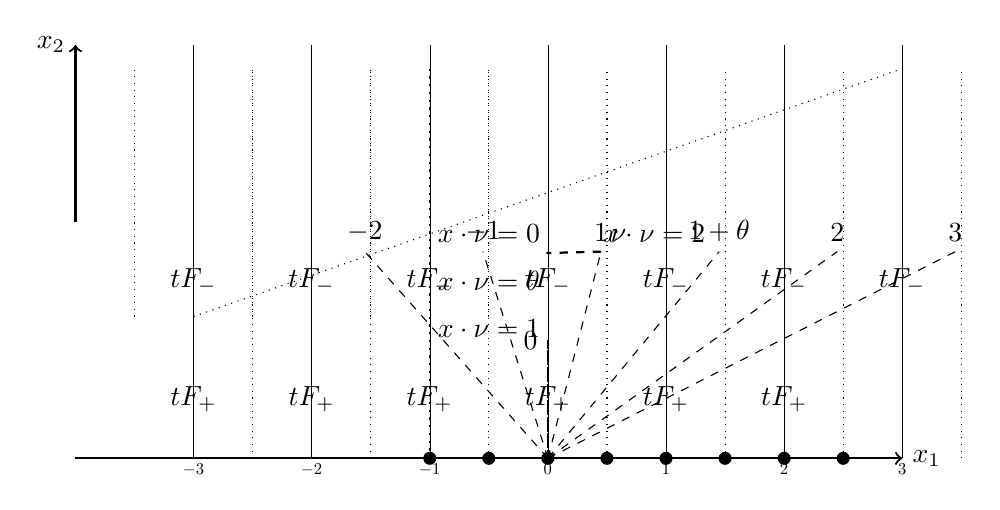
\begin{tikzpicture}[scale=1.5]
    \draw[->,thick] (-4,-1)--(3,-1) node[right]{$x_1$};
    \draw[->,thick] (-4,1)--(-4,2.5) node[left]{$x_2$};
    
    \foreach \x in {-3,-2,...,3}{%
        \draw[very thin] (\x,-1)--(\x,2.5);%
        \node[scale=.6,below] at (\x,-1){$\x$};%
    }
    
    \draw[dashed,thick] (0,-1)--(0,0) node[left]{$0$} ;
    
    \draw[dashed] (0,-1)--(-2+.75*.6,.75+.6-.6) node[above]{$-2$} ;
    \draw[dashed] (0,-1)--(-1+.75*.6,.75+.6-.6) node[above]{$-1$} ;
    \draw[dashed] (0,-1)--(.75*.6,.75+.6-.6) node[above]{$1$} ;
    \draw[dashed] (0,-1)--(1+.75*.6,.75+.6-.6) node[above]{$1+\theta$} ;
    \draw[dashed] (0,-1)--(2+.75*.6,.75+.6-.6) node[above]{$2$} ;
    \draw[dashed] (0,-1)--(3+.75*.6,.75+.6-.6) node[above]{$3$} ;
    
    \draw[dashed] (0,0)--(0,-1);
    
    \draw[dashed,thick] (.75*.6,.75+.6-.6)--(.75*.6,.75+.6-.6+.75*.6,.75+.6-.6+.75*.6);
    \node[anchor=south west] at (.75*.6,.75+.6-.6){$\nu$};
    
    \foreach \x in {-2.5,-1.5,...,3.5}{%
        \draw[dotted] (\x,-1)--(\x,.2);%
        \draw[dotted] (\x,-1)--(\x,2.5-.2);%
    }
    
    \draw[dotted] (-3,.2)--(3,2.5-.2);%
    
    \draw[dotted,thick] (-1,-1)--(-1,.2);%
    \draw[dotted,thick] (-1,-1)--(-1,2.5-.2);%
    
    \draw[dotted] (-3.5,.2)--(-3.5,2.5-.2);%
    \draw[dotted] (-2.5,.2)--(-2.5,2.5-.2);%
    \draw[dotted] (-1.5,.2)--(-1.5,2.5-.2);%
    \draw[dotted] (-.5,.2)--(-.5,2.5-.2);%
    
    \foreach \x in {-1,-.5,...,2.5}{%
        \node[circle,fill=black,scale=.5] at (\x,-1){};%
    }
    
    \node[scale=1.] at (-3,.5){$tF_-$};
    \node[scale=1.] at (-3,-.5){$tF_+$};
    \node[scale=1.] at (-2,.5){$tF_-$};
    \node[scale=1.] at (-2,-.5){$tF_+$};
    \node[scale=1.] at (-1,.5){$tF_-$};
    \node[scale=1.] at (-1,-.5){$tF_+$};
    \node[scale=1.] at (0,.5){$tF_-$};
    \node[scale=1.] at (0,-.5){$tF_+$};
    \node[scale=1.] at (1,.5){$tF_-$};
    \node[scale=1.] at (1,-.5){$tF_+$};
    \node[scale=1.] at (2,.5){$tF_-$};
    \node[scale=1.] at (2,-.5){$tF_+$};
    \node[scale=1.] at (3,.5){$tF_-$};
    
    \node[scale=1.] at (-.5,.9){$x\cdot\nu=0$};
    \node[scale=1.] at (-.5,.5){$x\cdot\nu=\theta$};
    \node[scale=1.] at (-.5,.1){$x\cdot\nu=1$};
    \node[scale=1.] at (.9,.9){$x\cdot\nu=2$};
    
    \end{tikzpicture}

\end{document}